%************************************************
\chapter{A Case Study: Foramide Chemistry}
\label{ch:casestudy1} %
%************************************************

{\sffamily\slshape The text in this chapter is identical to Section 4 of the published version of the preprint at \href{https://arxiv.org/abs/2411.15900}{arXiv:2411.15900}.\\}

In this chapter, we demonstrate the methods from Chapter~\ref{ch:thermodynamic_model} on a reaction network involving hydrogen cyanide, formamidic acid, and formamide in aqueous solution which has been studied in \cite{implemented_CRN}.

\section{Network Generation}

The reaction network was generated using M{\O}D by the expansion of the molecular space with the input molecules HCN, NH$_3$, and H$_2$O, by the recursive application of the graph transformation rules listed in Figure~\ref{fig: graphTransformationRules}.
The individual molecules in the generated network, such as HCN, NH$_3$, H$_2$O, formamide and so on, are represented as undirected labeled graphs.
\footnote{The atoms represented as vertices, labeled by the symbol of the element it represents, such as $C$ for a carbon atom, $H$ for a hydrogen atom, $N$ for a nitrogen atom, $O$ for an oxygen atom and so on. The bonds are represented as edges, labeled by bond types such as a single, double, triple or aromatic bond. The default bondtype is single.}
Stereo-information is not represented. Therefore, both the stereoisomers of the molecule shown in Figure~\ref{fig: molGraphs} are represented by the same graph. Hence, they cannot be distinguished in our modeling despite them being two different chemical entities.
Molecular graphs also constitute the vertices of the hypergraph representing the reaction network. 

\begin{figure}[b]
	\centering
    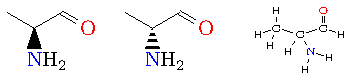
\includegraphics[scale=1.5]{graphics/chapter3/molGraphs.pdf}
    \vspace{0.2cm}
    \caption{Two stereoisomers of a molecule (left) and the corresponding molecular graph (right).}
    \label{fig: molGraphs}
\end{figure}

\begin{figure}[!t]
    \centering
    \begin{subfigure}{\textwidth}
        \centering
        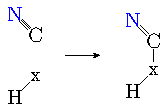
\includegraphics[scale=1.5]{graphics/chapter3/rule0.pdf}
        \vspace{0.2cm}
        \caption{Addition to a cyanide: in this rule \texttt{x} $\in$ \{N, O\}, representing the addition of an amide nitrogen or hydroxyl oxygen to the nitrile bond respectively.}
        \label{fig:rule0}
    \end{subfigure}
    \\
    \vspace{0.5cm}
    \begin{subfigure}{\textwidth}
        \centering
        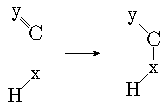
\includegraphics[scale=1.5]{graphics/chapter3/rule1.pdf}
        \vspace{0.2cm}
        \caption{Addition to an imine or carbonyl: in this rule \texttt{x}, \texttt{y} $\in$ \{N, O\}, representing the addition of an amide nitrogen or hydroxyl oxygen to an amide or hydroxyl bond respectively. This single rule encapsulates $2^2 = 4$ individual rules depending on the instantiation of \texttt{x} and \texttt{y}.}
        \label{fig:rule1}
    \end{subfigure}
    \\
    \vspace{0.5cm}
    \begin{subfigure}{\textwidth}
        \centering
        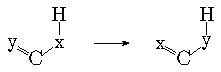
\includegraphics[scale=1.5]{graphics/chapter3/rule2.pdf}
        \vspace{0.2cm}
        \caption{1,3 hydrogen shift: in this rule \texttt{x}, \texttt{y} $\in$ \{C, N, O\}, representing the shift of a double bond as in tautomerism. When \texttt{x}$\equiv$O and \texttt{y}$\equiv$O it is keto-enol tautomerism, \texttt{x}$\equiv$N and \texttt{y}$\equiv$N is imine-enamine tautomerism, \texttt{x}$\equiv$N and \texttt{y}$\equiv$O is amine-iminol tautomerism and \texttt{x}$\equiv$C and \texttt{y}$\equiv$C is an allylic shift of the double bond. This single rule encapsulates $3\times 3 = 9$ individual rules depending on the instantiation of \texttt{x} and \texttt{y}.}
        \label{fig:rule2}
    \end{subfigure}%
    \\
    \vspace{0.5cm}
    \begin{subfigure}{\textwidth}
        \centering
        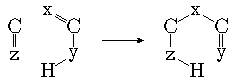
\includegraphics[scale=1.5]{graphics/chapter3/rule3.pdf}
        \vspace{0.2cm}
        \caption{Condensation: in this rule \texttt{x} $\in$ \{C, N, O\}, \texttt{y},\texttt{z} $\in$ \{N, O\} representation of the addition of a double bond (of an enol, enamine) to a imine or a carbonyl group. This single rule encapsulates $3\times 2\times 2 = 12$ individual rules depending on the instantiation of \texttt{x}, \texttt{y} and \texttt{z}.}
        \label{fig:rule3}
    \end{subfigure}%
    \vspace{0.5cm}
    \caption{The graph transformation rules used to expand the molecular space and generate the network.}
    \label{fig: graphTransformationRules}
\end{figure}

\begin{figure}[!h]
	\centering
	\vspace{0.5cm}
    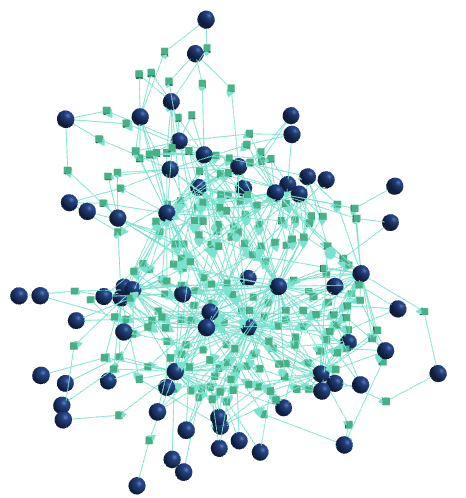
\includegraphics[width=0.8\textwidth]{graphics/chapter3/reactionNetworkChapter3.png}
    \vspace{0.5cm}
    \caption{An abstract representation of the generated reaction network with $67$ vertices (blue circles) and $202$ hyperedges (green squares), on which the working of the method proposed in Chapter~\ref{ch:thermodynamic_model} was demonstrated.}
    \label{fig: hypergraphRNChapter3}
\end{figure}

The graph transformation rules in Figure~\ref{fig: graphTransformationRules} represent classes of reactions, i.e. reaction templates. The left hand side of the rules is a subgraph, which may be substituted by the subgraph on the right hand side, when a match has been found in a molecular graphs present in the reaction network. This executes a reaction, thereby expanding the molecular space. Following the previous study of the network \cite{implemented_CRN}, the expansion was constrained to only generate molecules with a maximum of three carbon, three nitrogen, and three oxygen atoms. Moreover, only stable molecules ($x_v^{G^0} \leq 0$) were kept. 
The generated reaction network consists of $67$ vertices and $202$ hyperedges, and is shown in Figure~\ref{fig: hypergraphRNChapter3} for completeness.
A list of all molecules and transitions in the reaction network can be found in the associated GitHub repository \cite{data_repository}.

\section{Thermodynamic Oracle}
\label{sec:oracle} %

\begin{figure}[!t]
	\centering
    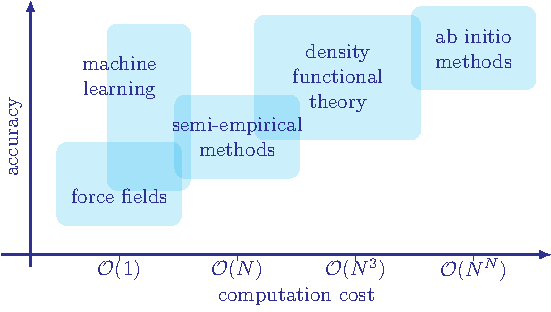
\includegraphics[width=0.8\textwidth]{graphics/chapter3/compCostCC.pdf}
    \vspace{0.5cm}
    \caption{A comparison of the computational costs of the available methods often used to assign free energies to molecules along with their accuracy. The rough ranges for the data used to draw the figure was collated from~\cite{ccCost}.}
    \label{fig: compChemCost}
\end{figure}

Given a reaction network, we assign chemical potentials to the molecules using what we had earlier referred to as a `thermodynamic oracle' in Chapter~\ref{ch:thermodynamic_model}. Utilizing quantum mechanical methods based on density functional theory (DFT) as this `thermodynamic oracle' quickly becomes impractical as the number of electrons in the molecule (denoted by $N$) increases, as indicated by the comparative computational costs of the different available methods as shown in Figure~\ref{fig: compChemCost}.
Calculating the electron density in a molecule using DFT is an iterative process. Each step invokes gradient descent, which scales beyond $\mathcal{O}(N^3)$ for classical DFT based methods for a single-point calculation because it involves matrix inversions. After the electron density for the molecule has been optimized, it can then be used to calculate the electronic contribution to the energy of a molecule.
Machine learnt relations for potential assignment exist, some require optimized atomic coordinates to determine potentials~\cite{NN_molecule_energies}, while others just utilize the connectivity of the molecular graph~\cite{ml_energy,ml_energy1,ml_energy2,ml_energy3} or even a string representation of it~\cite{ml-energy4}. However, these machine learnt relations from a dataset might not be well generalizable; they could perform poorly when a molecule sufficiently different, from those in the dataset trained on, is encountered~\cite{ml_energy5,ml_energy6,ml_energy7}. Ideally, kinetic rate parameters would have to be incorporated into the search for pathways in a reaction network as integer flows, because they dictate which reactions actually occur in the system and how fast. However, calculating activation free energies using DFT-based quantum mechanical methods to determine these kinetic parameters would demand even further time and computational resources.

\begin{figure}[!t]
	\centering
	\vspace{0.5cm}
    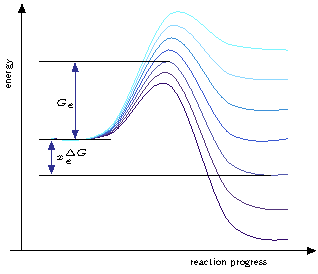
\includegraphics[width=0.8\textwidth]{graphics/chapter3/epsPrinciple.pdf}
    \vspace{0.5cm}
    \caption{In a group of not too diverse reactions, the energy barrier of a reaction can be considered to be dependent on the free energy change of the reaction by some function: $G_e = f\left(x_e^{\Delta G}\right)$. This holds because the reaction trajectories do not tend to cross each other when plotted normalized by the energy of the reactants.}
    \label{fig: epsPrinciple}
\end{figure}

As an alternative, we in this work adopt a compromise oracle based on equilibrium thermodynamics. This approximation has some theoretical basis behind it with the Evans– Polanyi–Semenov principle~\cite{epsPrinciple}, which states that within a class of reactions, the thermodynamics of the reaction acts as a proxy for the kinetics of the reaction, as shown in Figure~\ref{fig: epsPrinciple}. It allows us to substitute the energy barrier for a reaction with the free energy difference for a reaction resulting in the relation in Equation~\eqref{prob_transition}. Specifically, to balance accuracy, efficiency, generalizability, and running time, we employ a semi-empirical method, GFN2-xTB~\cite{grimme_xtb}, for potential assignment. While this method compromises on accuracy compared to DFT, the errors are acceptable for demonstrating the utility of the mathematical model on an example reaction network.
We detail the thermodynamic oracle we use to assign the chemical potentials to the molecules, $x_v^{G^0}$, in the reaction network in the following section.
An advantage of this modular approach is that it provides the reader the freedom to substitute the proposed thermodynamic oracle with another tool, for example pre-trained neural networks, mapping a molecule to its chemical potential (or even the reactions to their kinetics parameters) depending on the desired accuracies and available computational resources.

\section{On assigning the Chemical Potentials}\label{first appendix}

One of the main enhancements to the thermodynamic modeling of reaction networks in this work is a more robust, transparent and generic method of assigning the chemical potentials under standard physical conditions for molecules, $x^{G^0}_v$,
compared to relying on thermodynamic databases such as (\url{https://pytfa.readthedocs.io/en/latest/thermoDB.html})
 using the group contribution method, to infer the free energy change for reactions, $x^{G^0}_e$, 
as done in~\cite{hatz_therm_python}.
Using quantum chemical methods to assign these chemical potentials quickly becomes computationally resource-intensive because the time complexity scales as $\mathcal{O}(N^3)$. The density-functional theory (DFT) calculations involve diagonalization of the $N\times N$ Hamiltonian matrix. 
The memory requirement scales as $\mathcal{O}(N^2)$ because of the number of two-electron integrals contributing to the energy of the system. Moreover, it is an iterative process which is repeated until an acceptable convergence criteria is reached.

\begin{figure}[!t]
    \centering
    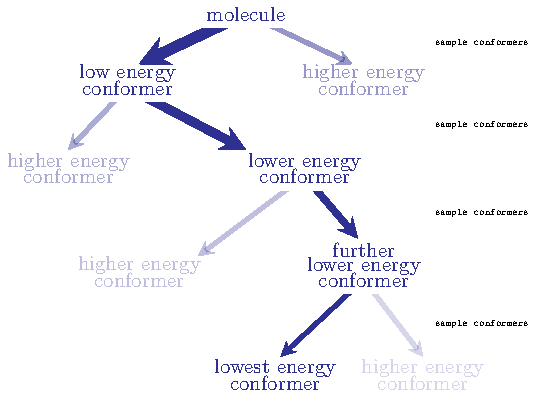
\includegraphics[width=0.9\textwidth]{graphics/chapter3/sampleConformer.pdf}
    \vspace{0.5cm}
    \caption{OpenBabel's \texttt{WeightetedRotorSearch()} iteratively samples conformers to reach towards the lowest energy conformer of the molecule. It randomly chooses from the allowed torsion angles, and reweights the choice based on the energy of the last generated lowest energy conformer. Progressively, the generated conformer has increasingly lower energy.}
    \label{fig: sampleConformer}
\end{figure}

Efficient software design necessitates striking a balance among the components in this work: expanding the molecular space, assigning chemical potentials to the molecules in the space and solving the formulated MILP for queried pathways in the network.   
If DFT calculations are employed, the calculation of chemical potentials required a significantly longer time compared to the remaining two components.
Alternative semi-empirical methods offered a faster yet reasonable accurate way to assign chemical potentials to molecules.
Therefore, we utilized xTB~\cite{grimme_xtb} to estimate the chemical potentials for the molecules in the expanded reaction network.
In the rest of this Section, we describe how we estimate the chemical potentials for the molecules from their representations as graphs which is aso illustrated in Scheme~\ref{fig: thermOracle}.

The molecules in the expanded reaction network were modeled as graphs where individual vertices represented atoms (labeled by the symbol of the corresponding element), while edges represented bonds. The adjacency matrix of this graph was utilized to determine the connectivity for that molecule. Given a connectivity matrix that satisfies the valences of each atom in the molecule, a three-dimensional embedding for the molecule was generated using the VSEPR theory. The \href{https://github.com/openbabel/openbabel/blob/32cf131444c1555c749b356dab44fb9fe275271f/include/openbabel/builder.h#L42}{\texttt{OBBuilder}} class from the Open Babel~\cite{open_babel, openbabel_web} library was employed to generate the three dimensional coordinates for the atoms utilizing a combination of VSEPR rules and commonly encountered fragments.

The generated geometry of the molecule was refined using 1000 iterations of conjugate gradient descent or until the change in energy (in atomic units, calculated using the universal force field~\cite{uff}) between successive iterations is less than $10^{-4}$. Next, to identify a low energy conformer, \href{https://github.com/openbabel/openbabel/blob/32cf131444c1555c749b356dab44fb9fe275271f/src/forcefield.cpp#L1595}{\texttt{OBForceField::WeightedRotorSearch()}} was utilized to systematically perform a tree-search for a conformer of the molecule with a low energy, by biasing the expansion of the search tree towards the current low energy conformer as shown in Figure~\ref{fig: sampleConformer}. At each iterative expansion step, 25 conformers were generated, and 100 steps of conjugate descent are executed on each. This lead to the generation of conformers with successively lower energies over subsequent iterations. The conformer with the lowest energy identified at the end of this search process was further subjected to 250 iterations of conjugate descent or until the energy tolerance of $10^{-5}$ is reached. The energy for a conformer at each step was estimated using the universal force field~\cite{uff}. The result of this search process, the configuration of the low-energy conformer, containing the three dimensional Cartesian coordinate of each atom in the molecule was written into an \texttt{.xyz} file. 

\begin{figure}[!t]
    \centering
    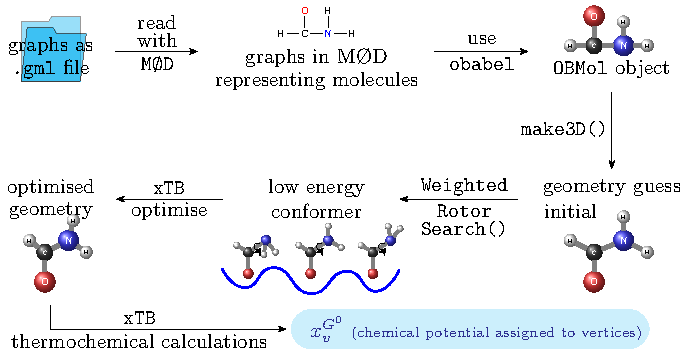
\includegraphics[width=1.1\textwidth]{graphics/chapter3/thermOracle.pdf}
    \vspace{0.5cm}
    \caption{The sequence of operations that was used to assign chemical potentials to the molecules, represented by vertices, in the reaction network, which is referred to thermodynamic oracle in the text.}
    \label{fig: thermOracle}
\end{figure}

The \texttt{.xyz} coordinate file generated by OpenBabel serves as an input file for xTB.
A geometry optimization of the structure is performed with xTB, employing an energy tolerance of $5\times 10^{-8}$ Eh and a gradient tolerance of $5\times 10^{-5}$ Eh bohr$^{-1}$. This is followed by the calculation of the Hessian matrix for the optimized structure, and the chemical potentials at $298.15$ K using standard translational, rotational, vibrational, and electronic partition functions from statistical mechanics under the coupled rigid-rotor and harmonic-oscillator approximations.

\section{On the range of the concentration variable}\label{second appendix}

Apart from the free energies for the molecules, $x^{G^0}_v$, assigned by the thermodynamic oracle the limits on the log concentration values of the molecules, $\left[x^K_v\right]_{\text{min}}$ and $\left[x^K_v\right]_{\text{max}}$ have to be assigned by the user. We provide some comments on the choice of these limits in this work. 
The upper limit for the concentrations is a physical limit bounded by the concentration of the pure substance. Concentration is expressed in the units of moles per liter (mol L$^{-1}$) for liquids and solutions while in terms of partial pressures (in Pa) for gases. For liquids, the maximum possible concentration value of the reactant would be that of the pure liquid, which is physically constrained by
\begin{align*}
    1 \text{ mol of pure liquid} &\equiv M \text{ kg of pure liquid} \\
    1 \text{ mol of pure liquid} &\equiv \frac{M}{\rho} \text{ L of pure liquid} \\
    \text{Maximum concentration} &\equiv \frac{\rho}{M} \text{mol L$^{-1}$}
\end{align*}
For gases, the maximum concentration is imposed by the physical constraint that it has to remain (an ideal) gas following the equation of state $PV = nRT$ so that the equations from the kinetic theory of gases might still be applied to it. The concentration of a gas under some given physical condition of pressure $P$ and temperature $T$ is
\begin{equation*}
    \frac{n}{V} = \frac{P}{RT}
\end{equation*}
As the pressure is increased, or the temperature is deceased to increase the concentration, the gas ceases to behave as an ideal gas and starts exhibiting properties of the vapor phase. A change in the physical state of the substance would have a free energy of phase reaction involved, and it can no longer be modeled only using the equations considered here. 

The lower limit of the reactants is imposed by practical constraints because there are limits to the dilution that can be achieved under laboratory conditions. For a solution, infinite dilution would lead to no solute (reactant) being present, and hence the reaction would not occur. For gases, there are lower limits to pressures that can be achieved in laboratory vacuum settings. Reactions occurring in the solid phase (or on surfaces) are governed by different physical equations and cannot be expressed by this framework. For all practical purposes, we can assume out reactants to be solutions or gases satisfying the condition of a well-stirred reactor.

For this work, we have chosen the limits in the concentration variables as $\left[x^K_v\right]_{\text{min}} = -3$ and $\left[x^K_v\right]_{\text{max}} = 1$. These correspond to physical values of the concentrations between $10^{-3}$ mol lit$^{-1}$ and $10^{1}$ mol lit$^{-1}$. While minimolar concentrations can be achieved under laboratory conditions using standard fludics procedures, a concentration of tens of molars is often encountered for pure liquids (the concentration of pure water is $55.56$ mol lit$^{-1}$). While we use the same range for the log concentration values for all the molecules in the reaction network, the user might choose to assign different ranges for different molecules to make the model more realistic.

\section{Formamide Chemistry}

The primary objective was to study the energetics of condensation pathways of the smaller seed molecules (HCN, NH$_3$, and H$_2$O) into larger oligomers, which might have implication for the prebiotic synthesis of amino acids and compare it with the pathways reported in \cite{implemented_CRN}. 
Therefore, the formulated MILP model was set up to query the pathways with HCN, NH$_3$, and H$_2$O as the input molecules and the trimer of formamide (numbered $17$ in \cite{implemented_CRN}) as the target molecule as shown in Figure~\ref{fig: pathwayQuery}.
The formulated MILP to search for pathways with the given input and output vertices had $336$ variables.

\begin{figure}[!t]
    \centering
    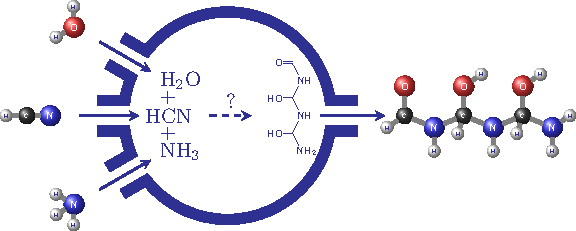
\includegraphics[width=\textwidth]{graphics/chapter3/queryPathway.pdf}
    \vspace{1.0cm}
    \caption{In the generated network, pathways to the target molecule, a trimer of formamide, were queries to with hydrogen cyanide, water and ammonia and source molecules using the method elaborated in Chapter~\ref{ch:thermodynamic_model}.}
    \label{fig: pathwayQuery}
\end{figure}

As a sanity check, the enumerated list of flow solutions returned by the solver included the pathway suggested in \cite{implemented_CRN}, thought not as the optimal solution when scored according to Equation~\eqref{obj_func_impl}.
The sum of free energies of the transitions in this pathway is $-178.412$ kJ mol$^{-1}$, while the sum of free energies weighted by the number of times it is used in the pathway yields $-405.332$ kJ mol$^{-1}$.
This pathway uses four unique transitions (hyperedges) as depicted in Figure~\ref{fig: conventional_path}.
Two of them are used multiple times, which makes seven transitions in total (sum of flows assigned to the hyperedges).
The pathway requires an inflow of three molecules of $v_0$ (hydrogen cyanide) and three molecules of $v_1$ (water) to produce the target molecule $v_5$. The chemical potential $x_v^{\Delta G}$ and the log concentration $x_v^K$ values assigned to each molecule by the MILP solver is listed in Table~\ref{tab:convSoln_molecules}, along with their molecular graphs. The free energy difference of the hyperedges used in the pathway along with the set of vertices which is the inset of the hyperedge (or the reactants in the corresponding transition) is listed under in($v$), while the set of vertices which is the outset of the hyperedge (or the products in the corresponding transition) is listed under out($v$) in Table~\ref{tab:convSoln_reactions}.
\clearpage

\begin{figure}[!t]
    \begin{subfigure}{\textwidth}
        \centering
        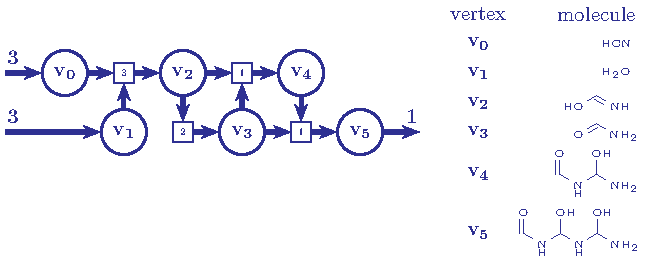
\includegraphics[scale=1.0]{graphics/chapter3/pathway1.pdf}
        \vspace{0.2cm}
        \caption{The pathway reported in \cite{implemented_CRN} with four hyperedges (with the assigned hyperflow the integer in the square) and the molecular graphs for the respective vertices.}
    \label{fig: conventional_path}
    \end{subfigure}
    \vspace{0.5cm}\\
    \begin{subfigure}{\textwidth}
        \centering
        \begin{footnotesize}
		\begin{tabular}{cccrr}
		    \\\toprule
		    vertex & inFlow & outFlow & $x_v^{\Delta G}$ & $x_v^K$ \\
		    \midrule
		    $v_0$ & $3$ & $0$ & $-5.507$ &  $1.000$ \\
		    $v_1$ & $3$ & $0$ & $-5.068$ & $-6.000$ \\
		    $v_2$ & $0$ & $0$ & $-10.610$ & $-6.000$ \\
		    $v_3$ & $0$ & $0$ & $-10.625$ & $0.195$ \\
		    $v_4$ & $0$ & $0$ & $-21.249$ & $-1.190$ \\   
		    $v_5$ & $0$ & $1$ & $-31.869$ & $-6.000$ \\
		    \bottomrule\\
		\end{tabular}
		\end{footnotesize}
		\caption{The inflow for the source molecules and the outflow of the target molecule, along with assignment of the chemical potentials, $x_v^{\Delta G}$, and log concentration, $x_v^K$, of the molecules in the pathway in Figure~\ref{fig: conventional_path}.}
		\label{tab:convSoln_molecules}
    \end{subfigure}
    \vspace{0.5cm}\\
    \begin{subfigure}{\textwidth}
        \centering
        \begin{footnotesize}
		\begin{tabular}{ccccr}
		    \\\toprule
		    hyperedge & $f_e$ & in($v$) & out($v$) & $\overline{x}^{\Delta G}_e$ \\
		    \midrule
		    $e_1$ & $3$ & $v_0, v_1$ & $v_2$ & $-94.141$ \\
		    $e_2$ & $2$ & $v_2$ & $v_3$ & $-38.629$ \\
		    $e_3$ & $1$ & $v_2, v_3$ & $v_4$ & $-0.006$ \\
		    $e_4$ & $1$ & $v_3, v_4$ & $v_5$ & $-45.645$ \\
		    \midrule
		    & & $\sum_e \overline{x}^{\Delta G}_e$ & $=$ & $-178.412$ \\
		    & & $\sum_e f_e\cdot \overline{x}^{\Delta G}_e$ & $=$ & $-405.332$ \\
		    \bottomrule\\
		\end{tabular}
		\end{footnotesize}
		\caption{The MILP solution assigns hyperflows $f_e$ to the hyperedges in the pathway from Figure~\ref{fig: conventional_path}.}
		\label{tab:convSoln_reactions}
    \end{subfigure}\\
    \vspace{0.5cm}
    \caption{Details of the pathway reported in \cite{implemented_CRN}. The $x_v^{\Delta G}$ values are in atomic units (Hartrees), the $x_v^K$ values are the dimensionless equivalent of $\log_{10} \frac{[\text{conc.}]}{1 \text{ mol lit}^{-1}}$, where conc. is the concentration of the molecule in mol lit$^{-1}$ while $\overline{x}^{\Delta G}_e$ are in kJ mol$^{-1}$.}
\end{figure}


\begin{figure}[!t]
    \begin{subfigure}{\textwidth}
        \centering
        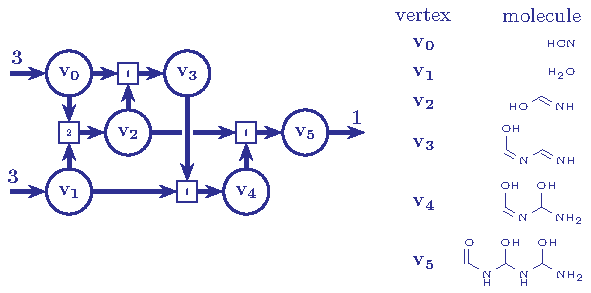
\includegraphics[scale=1.0]{graphics/chapter3/pathway2.pdf}
        \vspace{0.2cm}
        \caption{The best scoring pathway with four hyperedges and the molecular graphs for the respective vertices.}
    \label{fig: shortest_path}
    \end{subfigure}
    \vspace{0.5cm}\\
    \begin{subfigure}{\textwidth}
        \centering
        \begin{footnotesize}
		\begin{tabular}{cccrr}
		    \\\toprule
		    vertex & inFlow & outFlow & $x_v^{\Delta G}$ & $x_v^K$ \\
		    \midrule
		    $v_0$ & $3$ & $0$ & $-5.507$ &  $1.000$ \\
		    $v_1$ & $3$ & $0$ & $-5.068$ & $-6.000$ \\
		    $v_2$ & $0$ & $0$ & $-10.610$ & $1.000$ \\
		    $v_3$ & $0$ & $0$ & $-16.159$ & $-6.000$ \\
		    $v_4$ & $0$ & $0$ & $-21.240$ & $1.000$ \\        
		    $v_5$ & $0$ & $1$ & $-31.869$ & $-6.000$ \\
		    \bottomrule\\
		\end{tabular}
		\end{footnotesize}
    	\caption{The inflow for the source molecules and the outflow of the target molecule, along with assignment of the chemical potentials, $x_v^{\Delta G}$, and log concentration, $x_v^K$, of the molecules in the pathway in Figure~\ref{fig: shortest_path}.}
		\label{tab:shortestSoln_molecules}
    \end{subfigure}
    \vspace{0.5cm}\\
    \begin{subfigure}{\textwidth}
        \centering
        \begin{footnotesize}
		\begin{tabular}{ccccr}
		    \\\toprule
		    hyperedge & $f_e$ & in($v$) & out($v$) & $\overline{x}^{\Delta G}_e$ \\
		    \midrule
		    $e_1$ & $2$ & $v_0, v_1$ & $v_2$ & $-94.141$ \\
		    $e_2$ & $1$ & $v_0, v_2$ & $v_3$ & $-129.554$ \\
		    $e_3$ & $1$ & $v_1, v_3$ & $v_4$ & $-38.298$ \\
		    $e_4$ & $1$ & $v_2, v_4$ & $v_5$ & $-51.185$ \\
		    \midrule
		    & & $\sum_e \overline{x}^{\Delta G}_e$ & $=$ & $-313.178$ \\
		    & & $\sum_e f_e\cdot \overline{x}^{\Delta G}_e$ & $=$ & $-407.319$ \\
		    \bottomrule\\
		\end{tabular}
		\end{footnotesize}
		\caption{The MILP solution assigns hyperflows $f_e$ to the hyperedges in the pathway from Figure~\ref{fig: shortest_path}.}
		\label{tab:shortestSoln_reactions}
    \end{subfigure}\\
    \vspace{0.5cm}
    \caption{Details of the best scoring pathway on applying the model proposed in Chapter~\ref{ch:thermodynamic_model} along with the objective function (8). The units are the same as in Table~\ref{tab:convSoln_reactions}.}
\end{figure}

While thermodynamics might provide an insight to the equilibrium flows in the reaction network,
it does not describe the path to that equilibrium.
Each transition has an associated barrier energy that must be overcome for the transition to occur.
Enumerating pathways using our implementation of the MILP formulation of the problem provides the pathway in Figure~\ref{fig: shortest_path} as one with the minimum value of the objective function.
This pathway utilizes four unique transitions and five transitions in all to realize the pathway,
which is fewer than the previously reported pathway.
Since the difference in the chemical potential between the source and target molecules is fixed,
choosing hyperedges with larger free energy differences would increase the value of the objective function.
Using transition with larger free energy differences to `cover' the net difference in the chemical potential,
lead to fewer transitions being used in the pathway. 

The main source of difference in the objective function value in the two pathways is the chemical potential of the molecule $v_3$ from Figure~\ref{fig: shortest_path} that is not present in the conventional pathway.
While the conventional pathway in~\cite{implemented_CRN} is more symmetric and appealing because of the stepwise nucleophilic attack on the carbonyl $C$ atom by the amine $N$ atom of an adjacent $v_3$ molecule, which is repeated twice to generate $v_5$ as illutrated in Figure~\ref{fig: symAdd}, \cite{implemented_CRN} also notes that these condensation reactions have a positive Gibbs free energy.

\begin{figure}[!t]
	\begin{subfigure}{\textwidth}
        \centering
        \vspace{0.2cm}
        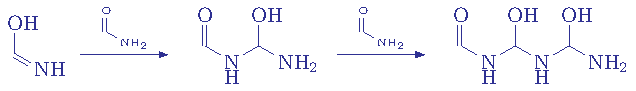
\includegraphics[scale=1.0]{graphics/chapter3/symAdd.pdf}
        \vspace{0.2cm}
    	\caption{Stepwise trimerization of formamide by iterative addition of the monomer as hypothesised in the conventional pathway shown in Figure~\ref{fig: conventional_path}.}
    	\label{fig: symAdd}
    \end{subfigure}\\
    \vspace{0.5cm}
    \begin{subfigure}{\textwidth}
        \centering
        \vspace{0.2cm}
        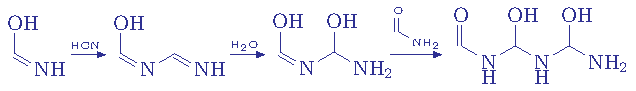
\includegraphics[scale=1.0]{graphics/chapter3/stepAdd.pdf}
        \vspace{0.2cm}
        \caption{The trimerization of formamide which uses $v_3$ in the pathway that is returned as the best scoring pathway as shown in Figure~\ref{fig: shortest_path}.}
        \label{fig: stepAdd}
    \end{subfigure}
    \caption{The difference between the best-scoring pathway returned by the proposed method and the pathway hypothesised in~\cite{implemented_CRN}.}
\end{figure}

To quote the authors, 
\begin{quote}
`\emph{each step is endergonic although decreasingly so.
Dimerization of formamide is uphill 19.8 kcal/mol, owing to the thermodynamic stability of the monomers in solution.
Addition of another monomer to form the trimer, via similar nucleophilic attack, is uphill 19.0 kcal/mol}'.
\end{quote}
This can also be observed in the ILP solution in Table~\ref{tab:convSoln_reactions} for the conventional pathway where the hyperedges $e_3 \equiv (\{v_2, v_3\}, \{v_4\})$ have a $\overline{x}_e^{\Delta G}$ value close to zero.
The constraint in Equation~\eqref{proposed_constraint3} forces the hyperedge to have $\overline{x}_e^{\Delta G} \leq 0$ for it to be included in the pathway.
The MILP solver chooses the log concentration variables $x_v^K$ for the molecules $v_3$ and $v_4$ in such a way so that $\overline{x}_e^{\Delta G}$ variables for $e_3$ is just below zero to realize the pathway.
This might be the reason for $x_v^K$ for these two vertices not having the extremal value as is often the case, as discussed below.
Our proposed model also returns an alternative pathway involving $v_3$ from Figure~\ref{fig: stepAdd}, where none of the $\overline{x}_e^{\Delta G}$ weights for the hyperedges is close to zero as listed in Table~\ref{tab:shortestSoln_reactions}.

We observe that the log concentration variables are always assigned extremal values decided by the constraint in Equation~\eqref{proposed_constraint8}.
This is likely an artifact of using an MILP solver with an objective function for the problem.
An MILP is a convex optimization problem where minimizing the objective function (involving a subset of the MILP variables) results in a solution located at a vertex of the convex space defined by the constraints.
The bounds for the variables are hand-crafted by the user and it might be more realistic to assign different bounds for the log concentration variable for each vertex.
Alternatively, a better interpretation of the assigned values for the variables, $x_v^K$ might be the direction in which the equilibrium concentrations have to be perturbed to achieve the desired flow.
For example, the concentration values in Table~\ref{tab:convSoln_molecules} can be interpreted as the concentrations of $v_1$, $v_3$ and $v_5$ have to be lowered and the concentrations of $v_0$, $v_2$ and $v_4$ have to be raised to achieve a larger difference in the potentials while effecting a net outflow of molecule $v_5$ given input molecules $v_0$ and $v_1$. 

\begin{table}[!t]
    \centering
    \begin{footnotesize}
    \begin{tabular}{ccccrrr}
        \\\toprule
        \# & $\sum_{e} f_e$ & $\sum_{e} z_e$ & $|v|$ & \hspace{0.1cm}obj \eqref{obj_func_impl} & $\sum_{e} f_e \cdot x_e^{\Delta G}$ & rxn sequence \\
        \midrule
        0 & $5$ & $4$ & $6$ & $-305.697$ & $-399.837$ & $1,3,4,10$ \\
        1 & $6$ & $5$ & $7$ & $-306.697$ & $-399.837$ & $1,3,4,5,9$ \\
        2 & $6$ & $5$ & $7$ & $-305.696$ & $-399.836$ & $1,2,3,4,11$ \\

		3 & $5$ & $3$ & $5$ & $-211.555$ & $-399.836$ & $1,6,9$ \\   
		4 & $5$ & $3$ & $5$ & $-211.554$ & $-399.836$ & $1,8,10$ \\
		5 & $6$ & $4$ & $6$ & $-211.556$ & $-399.836$ & $1,8,5,9$ \\
        6 & $6$ & $4$ & $6$ & $-211.556$ & $-399.836$ & $1,2,7,9$ \\     
        7 & $6$ & $4$ & $6$ & $-211.554$ & $-399.836$ & $1,2,8,11$ \\
        \bottomrule\\
    \end{tabular}
    \end{footnotesize}
    \caption{All enumerated pathways to the target molecule in the network, with the sequence of pathways leading to the target molecules. The specific reactions corresponding to the index listed in the sequence of reactions for each pathway listed in the last column can be read from Figure~\ref{fig: rxnList}. }
    \label{tab: thermo_flow}
\end{table}

An exhaustive search of the reaction space led to the identification of $13$ distinct reaction pathways \cite{solutions_data}, listed in Table~\ref{tab: thermo_flow} in the order of increasing value of objective \ref{obj_func_impl}. The column list the rank, the total number of reactions used, the number of unique reactions used, the number of molecules involved, the value of the objective \eqref{obj_func_impl} and the sum of the free energy differences of the reactions weighted by the flows in the columns respectively. Note, that the second column from the right gives the net free energy difference, which is path independent and therefore, the same for all the listed pathways. These pathways were enumerated in $866$ seconds on an AMD$^{\circledR}$ Ryzen 5 PRO 4650U CPU (2.1 GHz) utilizing $8$ threads. One may consult the list of reactions in Figure~\ref{fig: rxnList} for the molecules and the exact set of reactions involved in these pathways.

\begin{figure}[!t]
    \centering
    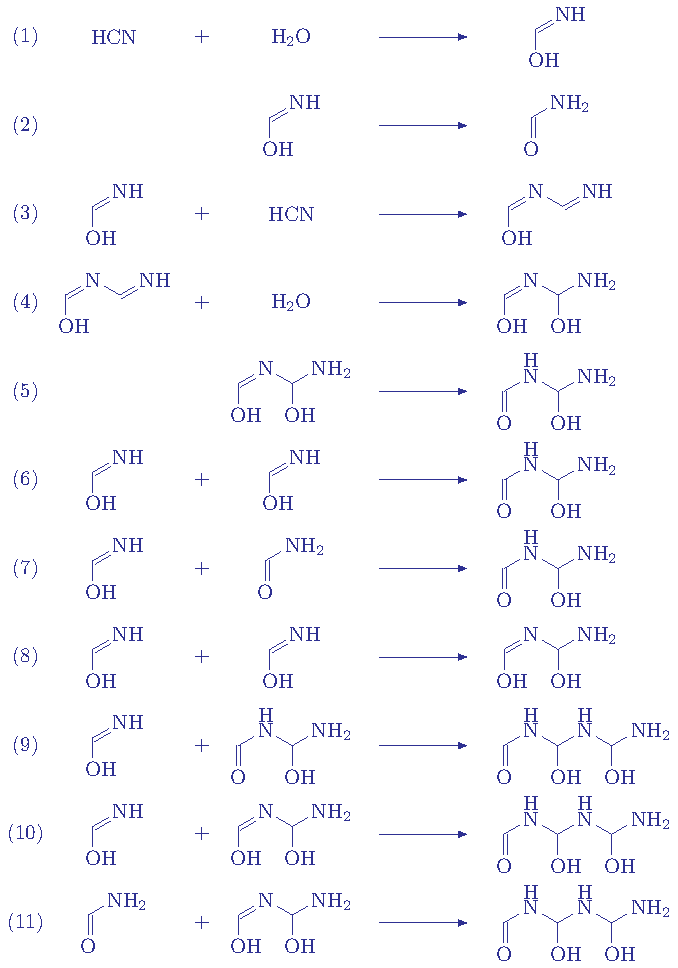
\includegraphics[scale=1.0]{graphics/chapter3/rxnList.pdf}
    \vspace{0.5cm}
    \caption{The list of the reactions used in the pathways to the target molecules, with the sequence of specific reactions in each pathway listed in Table~\ref{tab: thermo_flow}.}
    \label{fig: rxnList}
\end{figure}
